%%%%%%%%%%%%%%%%%%%%%%%%%%%%%%%%%%%%%%%%%%%%%%%%%%%%%%
% A Beamer template for HKUST (GZ)                   %
% Based on THU beamer theme                          %
% Author: Yuxuan HU                                  %
% Date: Aug 2024                                    %
% LPPL Licensed.                                     %
%%%%%%%%%%%%%%%%%%%%%%%%%%%%%%%%%%%%%%%%%%%%%%%%%%%%%%

\documentclass[serif, aspectratio=169]{beamer}
%\documentclass[serif]{beamer}  % for 4:3 ratio
\usepackage[T1]{fontenc} 
\usepackage{fourier} % see "http://faq.ktug.org/wiki/uploads/MathFonts.pdf" for other options
\usepackage{hyperref}
\usepackage{latexsym,amsmath,xcolor,multicol,booktabs,calligra}
\usepackage{graphicx,pstricks,listings,stackengine}
\usepackage{lipsum}
\usepackage{parskip}
\usepackage{amsmath}

\author{MAS}
\title{KANs and DeepOKANs}
\subtitle{Brief Introduction}
\institute{
    \\
    IISc, Bengaluru\\
}
\date{\small \today}
\usepackage{HKUSTstyle}

% defs
\def\cmd#1{\texttt{\color{red}\footnotesize $\backslash$#1}}
\def\env#1{\texttt{\color{blue}\footnotesize #1}}
% set colors
\definecolor{hkustyellow}{RGB}{167, 131, 55}
\definecolor{hkustblue}{RGB}{0, 56, 116}
\definecolor{hkustred}{RGB}{209, 51, 59}
\newcommand{\argmin}{\operatornamewithlimits{arg\,min}}


\lstset{
    basicstyle=\ttfamily\small,
    keywordstyle=\bfseries\color{deepblue},
    emphstyle=\ttfamily\color{deepred},    % Custom highlighting style
    stringstyle=\color{deepgreen},
    numbers=left,
    numberstyle=\small\color{halfgray},
    rulesepcolor=\color{red!20!green!20!blue!20},
    frame=shadowbox,
}

%- --- --- --- --- --- --- --- --- --- --- --- --- --- --- --- 
\begin{document}

\begin{frame}
    \titlepage
    \vspace*{-0.6cm}
    \begin{figure}[htpb]
        \begin{center}
            
\includegraphics[keepaspectratio, scale=0.02]{unilogo.png}
        \end{center}
    \end{figure}
\end{frame}

\begin{frame}
    \tableofcontents[sectionstyle=show,
        subsectionstyle=show/shaded/hide,
        subsubsectionstyle=show/shaded/hide]
\end{frame}

% Introduction --- --- --- --- --- --- --- --- --- --- --- --- 

\section{Introduction to Data Fitting}
\begin{frame}{Background and Motivation}
    \frametitle<presentation>{Representing Smooth Functions}
    %attaching a picture from umar jamil
    \begin{figure}
        \centering
        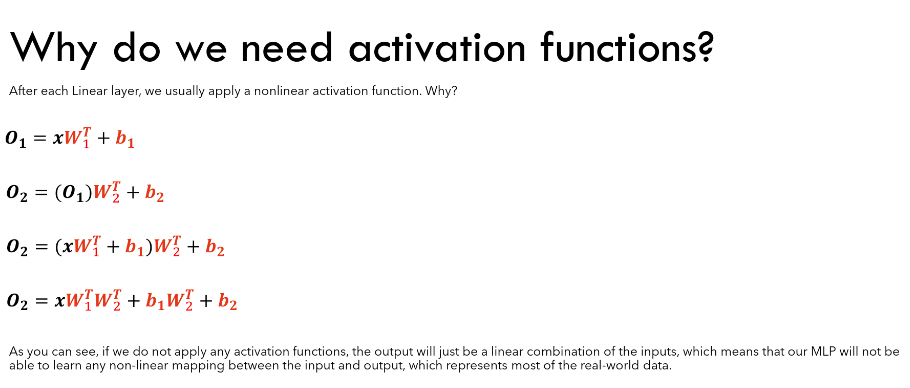
\includegraphics[height=6cm]{datafit.png}
    \end{figure}
    % \begin{block}{}
    %     \begin{itemize}
    %         \item show the main arguments and resuts of your work
    %         \item produce interest to read the full paper/report
    %         \item goal: be educational and also entertaining
    %     \end{itemize}
    % \end{block}
    % \begin{block}{Advantages of using \LaTeX ~with the beamer package:}
    %     \begin{itemize}
    %         \item very easy if the report is already written in \LaTeX
    %         \item different themes which are usable in practice
    %         \item possibility to create handouts using \emph{beamerarticle}
    %     \end{itemize}
    % \end{block}
\end{frame}

\begin{frame}{Background and Motivation}
    \frametitle<presentation>{Representing Smooth Functions}
    %attaching a picture from umar jamil
    \begin{figure}
        \centering
        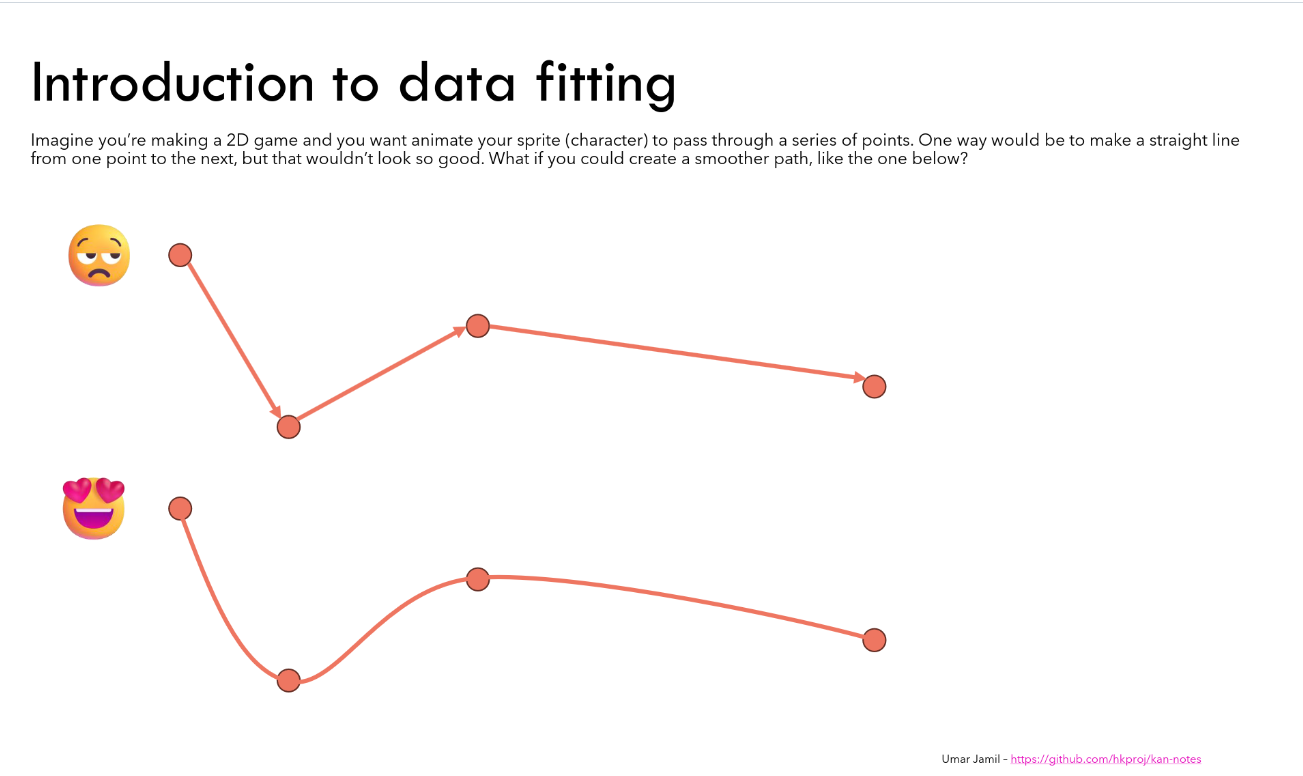
\includegraphics[height=7cm]{smooth.png}
    \end{figure}
\end{frame}
\begin{frame}{Background and Motivation}
    \frametitle<presentation>{Representing Smooth Functions}
    %attaching a picture from umar jamil
    \begin{figure}
        \centering
        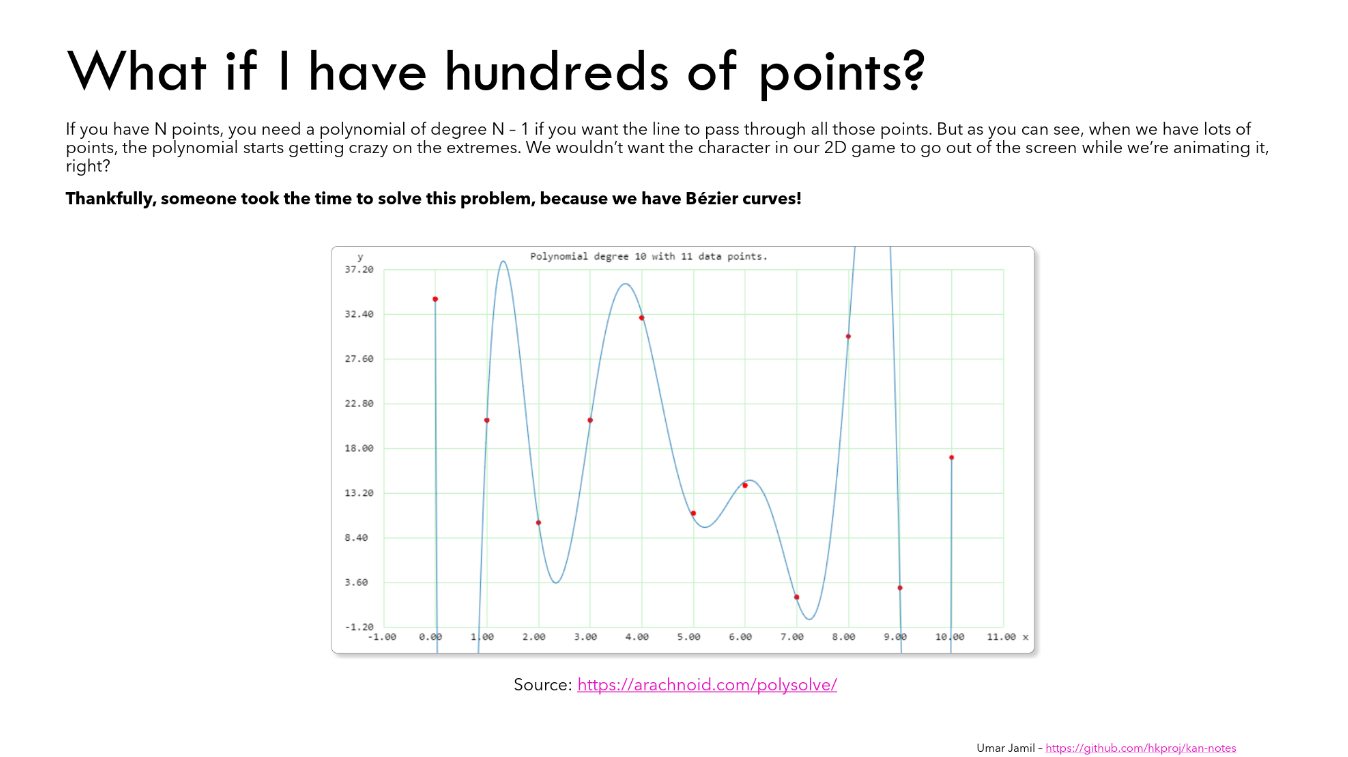
\includegraphics[height=7cm]{hund.png}
    \end{figure}
\end{frame}
\begin{frame}{Background and Motivation}
    \frametitle<presentation>{Representing Smooth Functions}
    %attaching a picture from umar jamil
    \begin{figure}
        \centering
        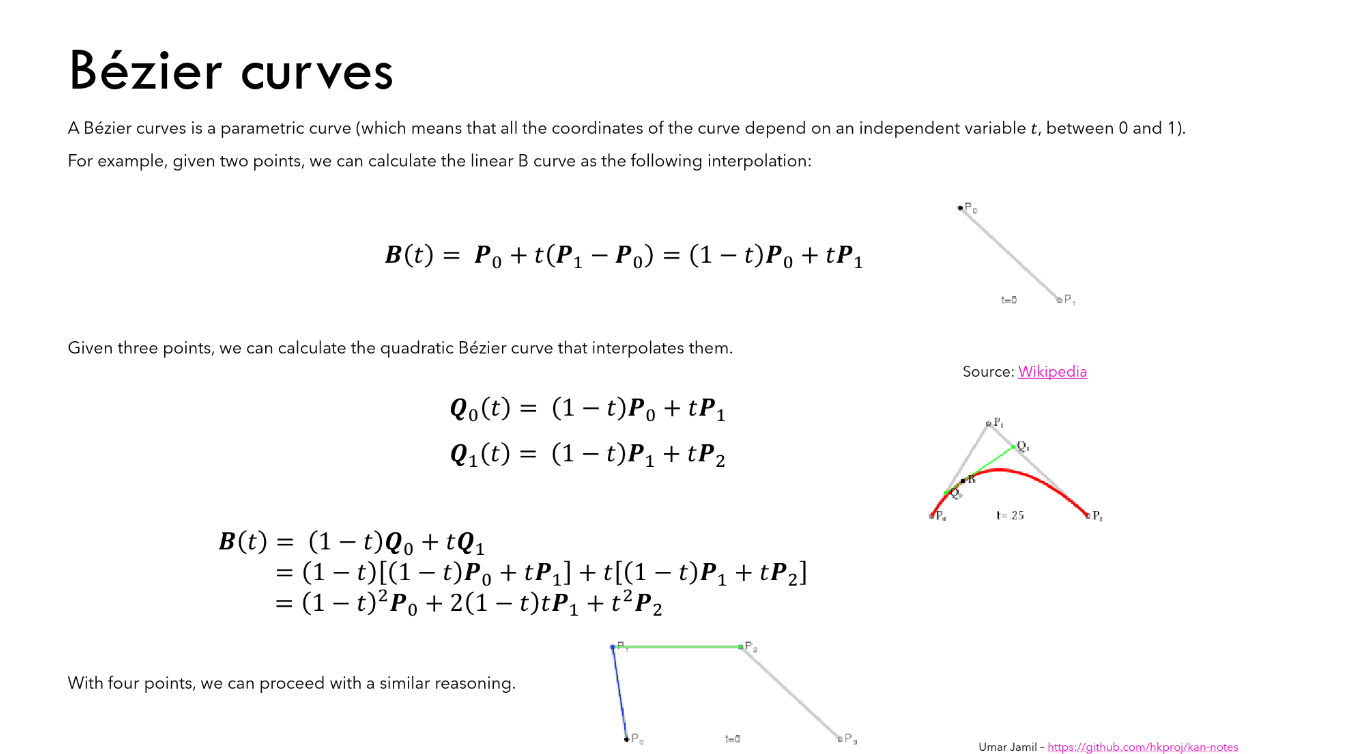
\includegraphics[height=7cm]{bezier.png}
    \end{figure}
\end{frame}
\begin{frame}{Background and Motivation}
    \frametitle<presentation>{Representing Smooth Functions}
    %attaching a picture from umar jamil
    \begin{figure}
        \centering
        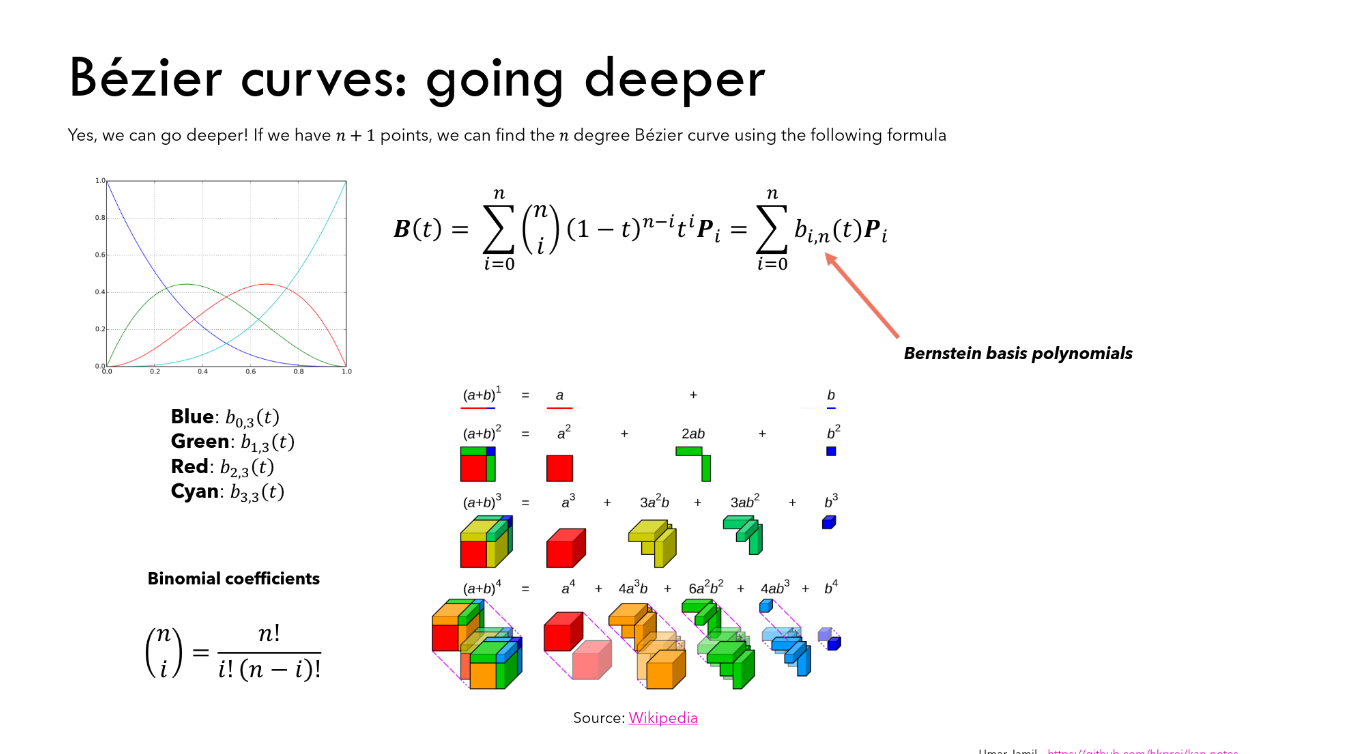
\includegraphics[height=7cm]{image.png}
    \end{figure}
\end{frame}
\begin{frame}{Background and Motivation}
    \frametitle<presentation>{Representing Smooth Functions}
    %attaching a picture from umar jamil
    \begin{figure}
        \centering
        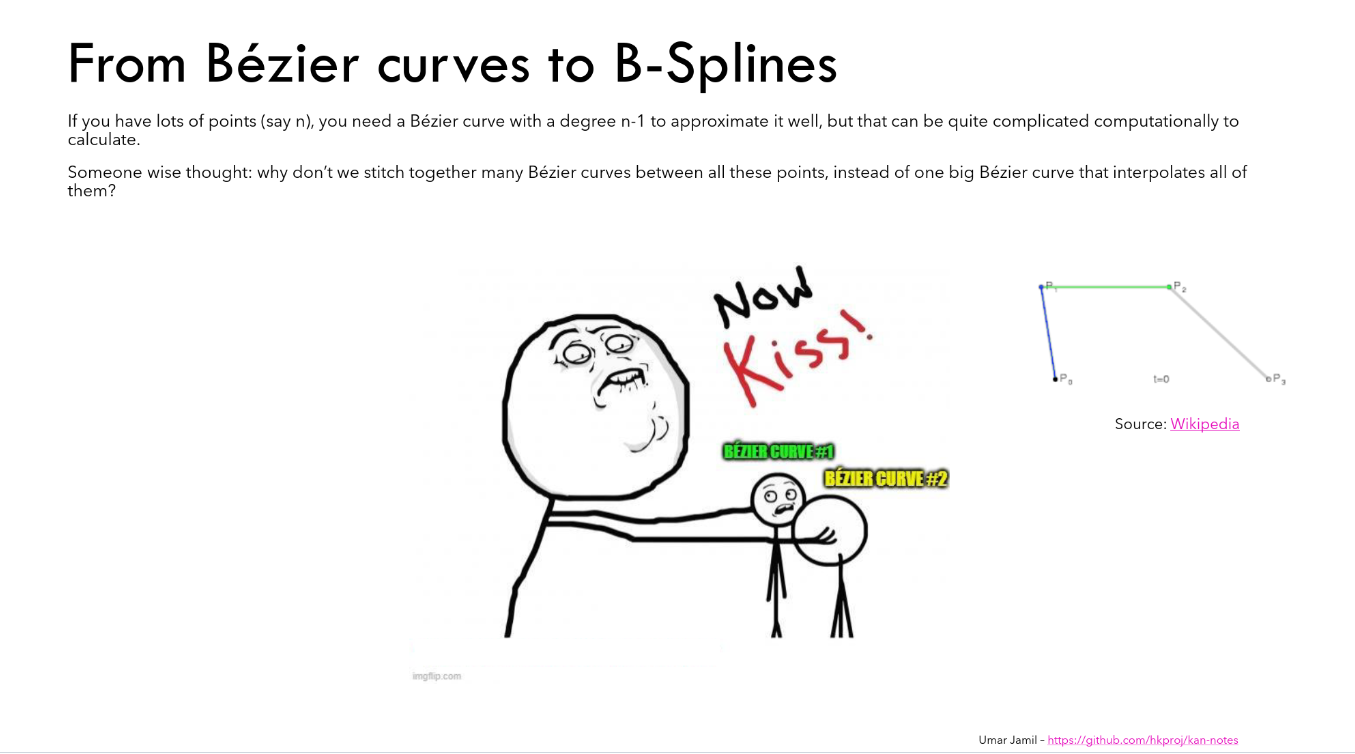
\includegraphics[height=7cm]{image copy.png}
    \end{figure}
\end{frame}
\begin{frame}{Background and Motivation}
    \frametitle<presentation>{Representing Smooth Functions}
    %attaching a picture from umar jamil
    \begin{figure}
        \centering
        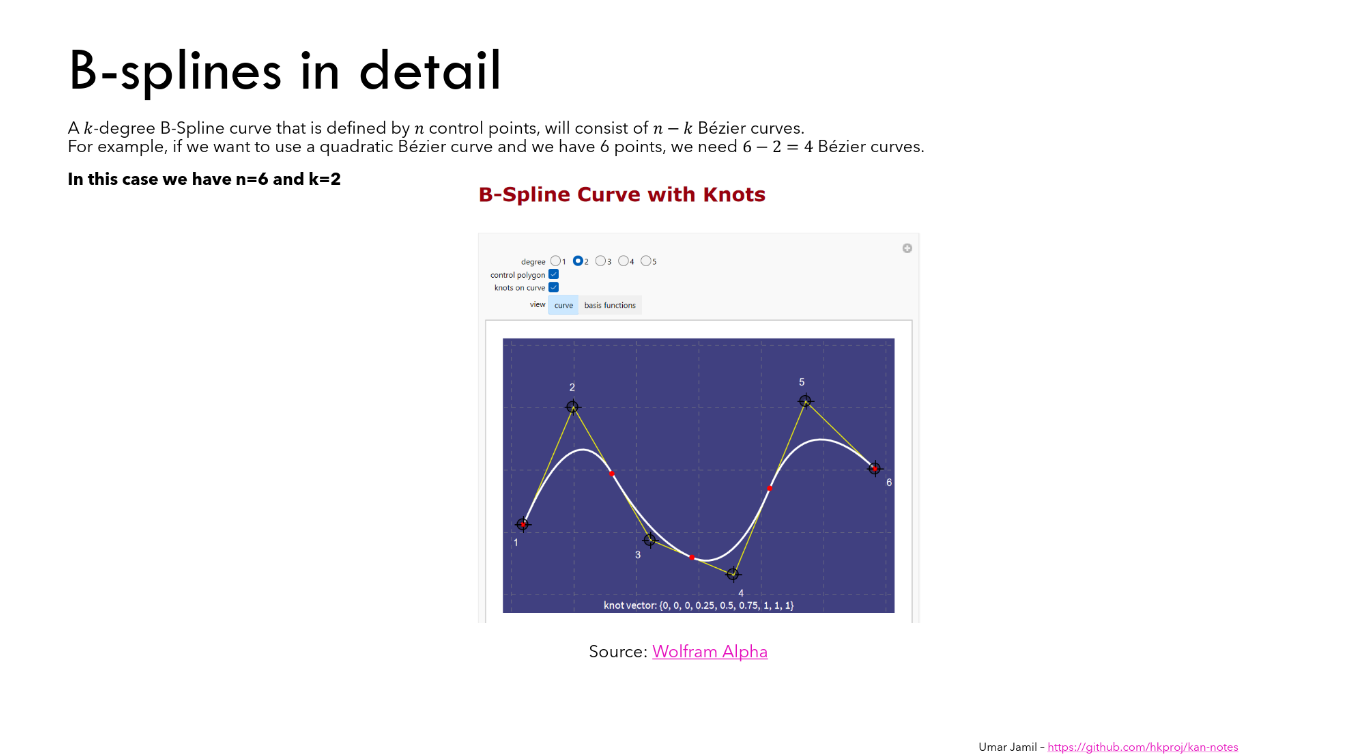
\includegraphics[height=7cm]{image copy 2.png}
    \end{figure}
\end{frame}
\begin{frame}{Background and Motivation}
    \frametitle<presentation>{Representing Smooth Functions}
    %attaching a picture from umar jamil
    \begin{figure}
        \centering
        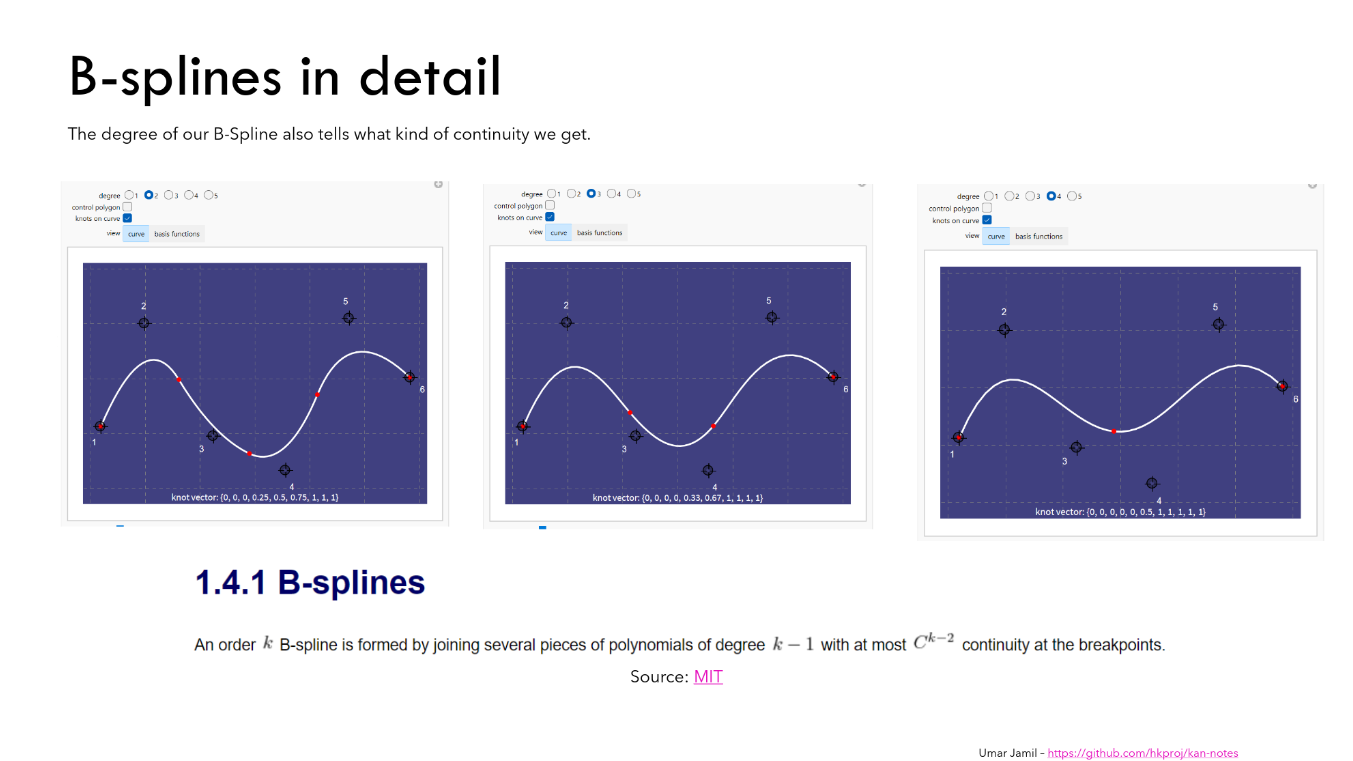
\includegraphics[height=7cm]{image copy 3.png}
    \end{figure}
\end{frame}
\begin{frame}{Background and Motivation}
    \frametitle<presentation>{Representing Smooth Functions}
    %attaching a picture from umar jamil
    \begin{figure}
        \centering
        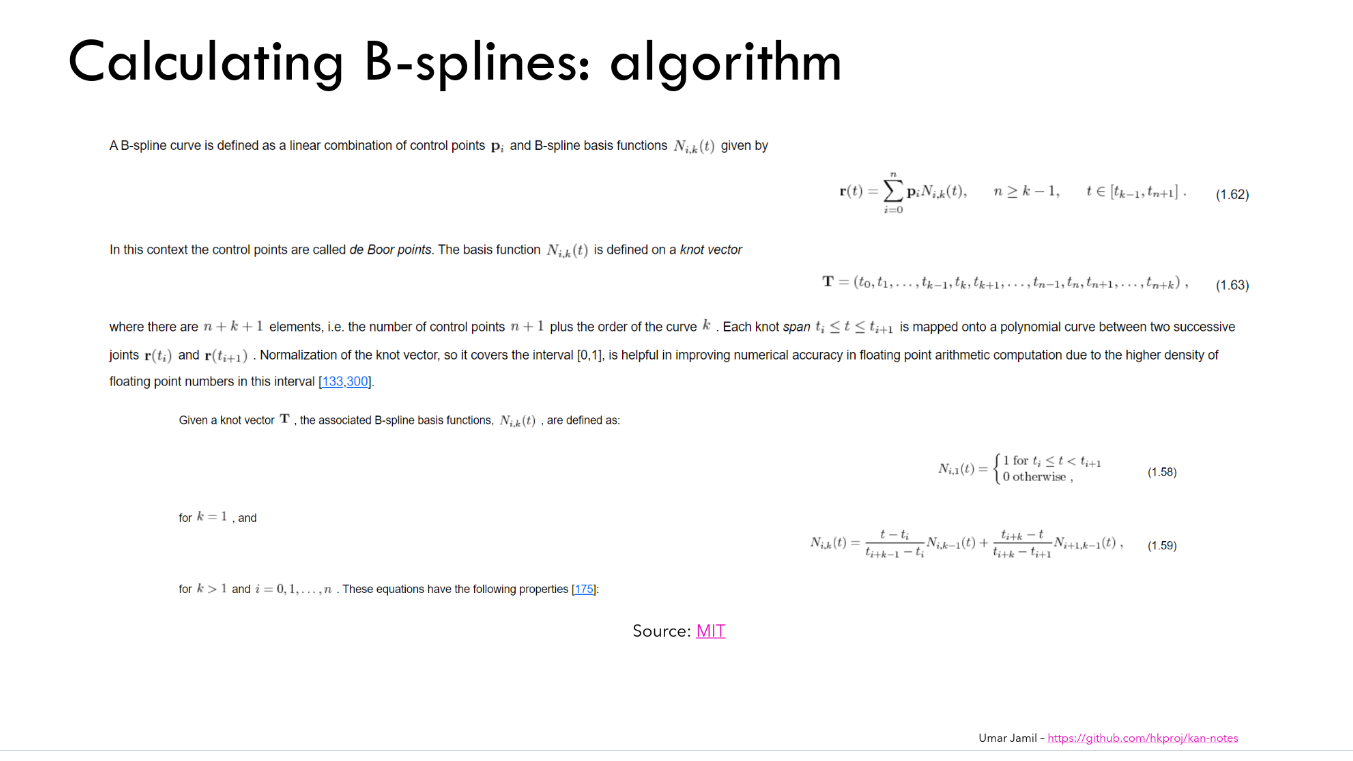
\includegraphics[height=7cm]{image copy 4.png}
    \end{figure}
\end{frame}
\begin{frame}{Background and Motivation}
    \frametitle<presentation>{Representing Smooth Functions}
    %attaching a picture from umar jamil
    \begin{figure}
        \centering
        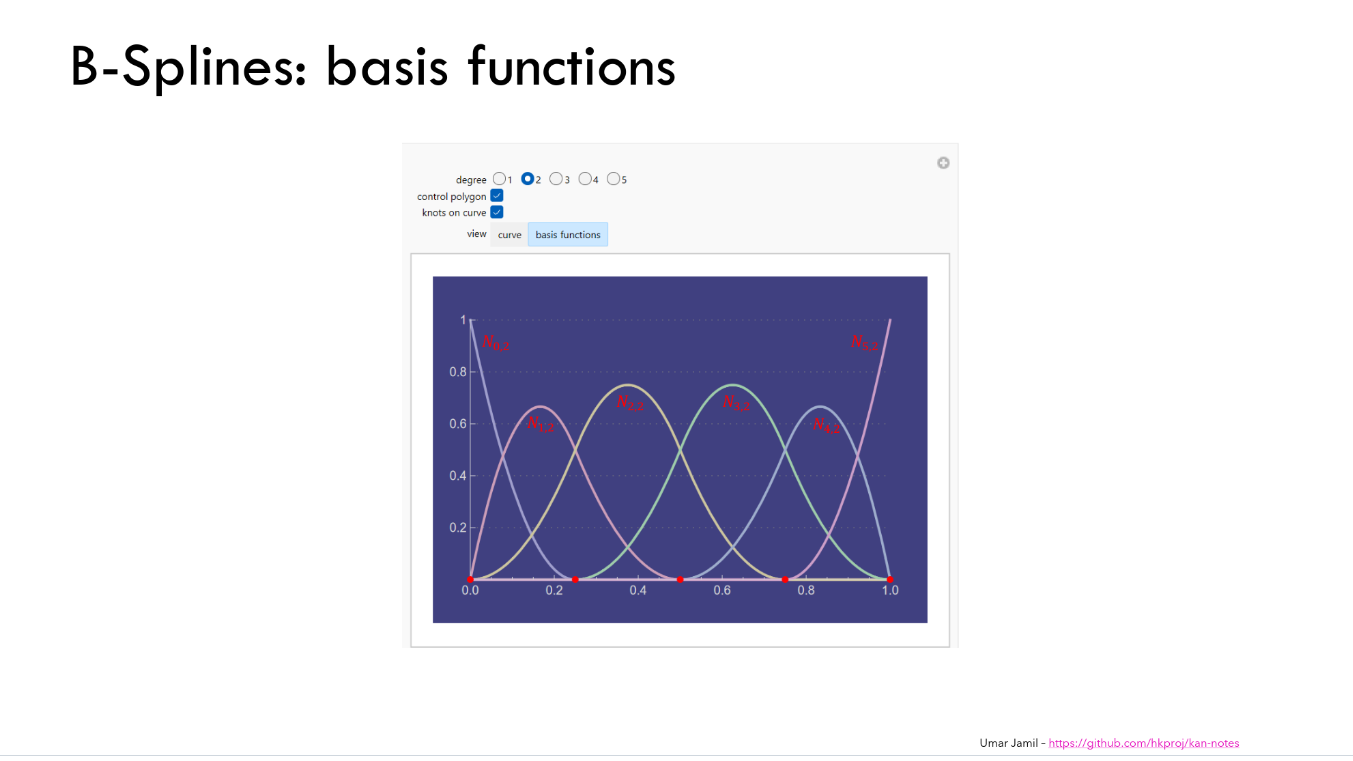
\includegraphics[height=7cm]{image copy 5.png}
    \end{figure}
\end{frame}
\begin{frame}{Background and Motivation}
    \frametitle<presentation>{Representing Smooth Functions}
    %attaching a picture from umar jamil
    \begin{figure}
        \centering
        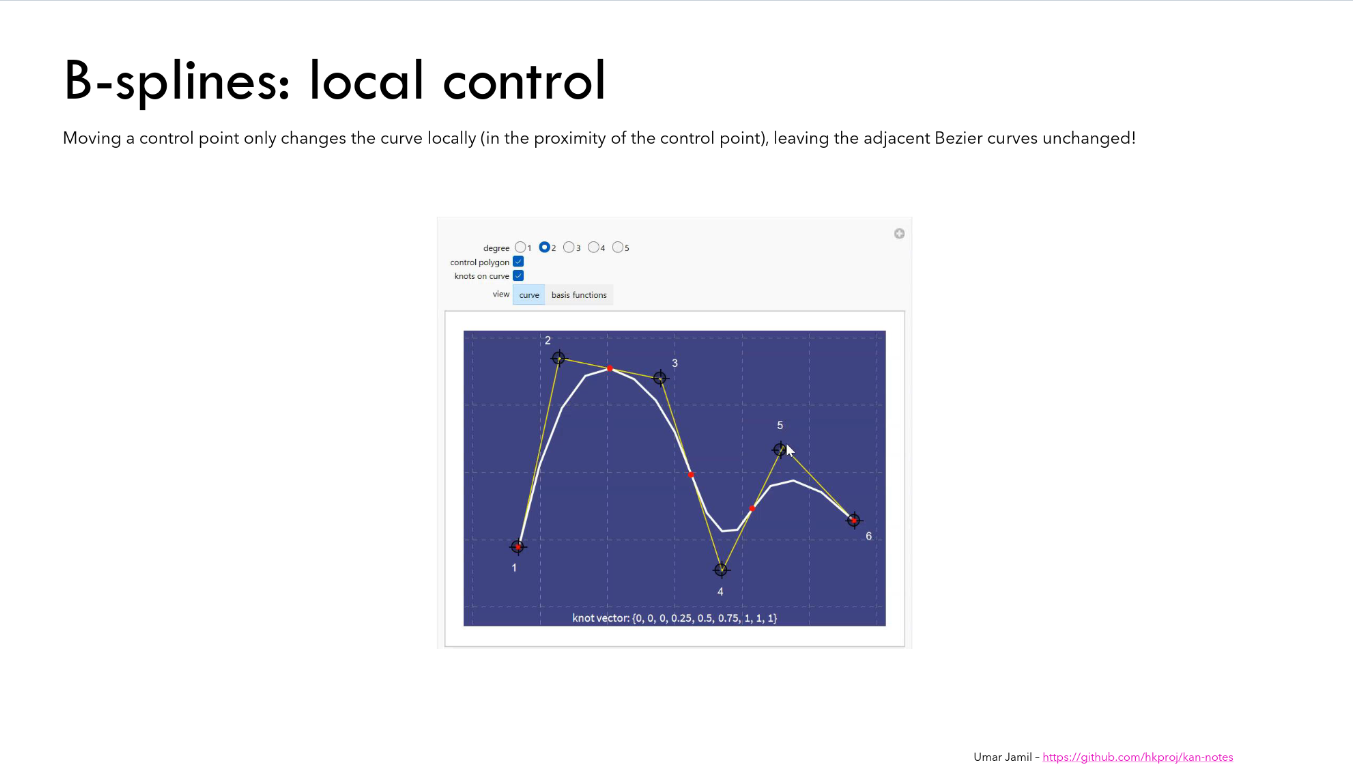
\includegraphics[height=7cm]{image copy 6.png}
    \end{figure}
\end{frame}
% Literature Review --- --- --- --- --- --- --- --- --- --- --- 
\section{Introduction to KAN}
\begin{frame}{Intro to KAN}
    \frametitle<presentation>{MLP vs KAN}
    %attaching a picture from umar jamil
    \begin{figure}
        \centering
        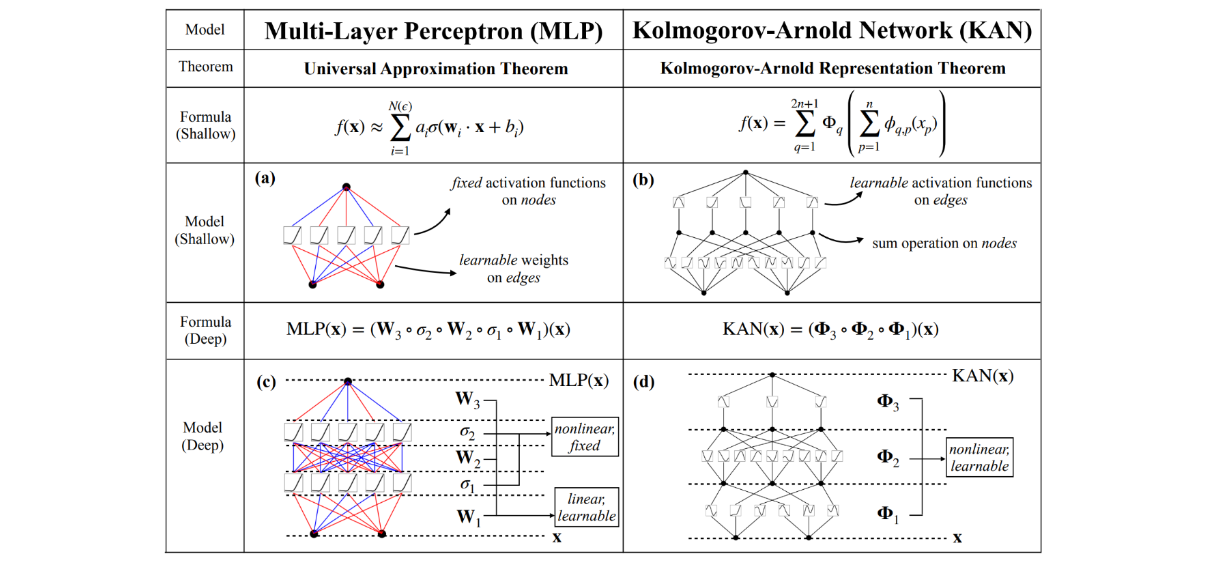
\includegraphics[height=6cm]{image copy 7.png}
    \end{figure}
\end{frame}
\begin{frame}{Intro to KAN}
    \frametitle<presentation>{Why KAN and not MLPs?}
    - \textbf{MLPs \& Nonlinear Approximation}: MLPs are widely used for nonlinear function approximation due to their expressive power (Universal Approximation Theorem), but they have drawbacks: low interpretability, less accuracy in low dimensions, and the curse of dimensionality (COD) in high dimensions.

    - \textbf{Introduction of KANs}: The paper introduces Kolmogorov-Arnold Networks (KANs), inspired by the Kolmogorov-Arnold representation theorem, as an alternative to MLPs.

    - \textbf{Previous Work}: Earlier research focused on depth-2, width-(2n + 1) networks, showing potential in breaking the COD empirically and theoretically, particularly with compositional function structures.

    - \textbf{New Approach}: This paper proposes deeper and wider network architectures, leveraging backpropagation for training, to enhance performance beyond the traditional depth-2, width-(2n + 1) representation.
\end{frame}
\begin{frame}{Intro to KAN}
    \frametitle<presentation>{KANs are a combo of MLPs and splines}
    - \textbf{Splines}: Accurate for low dimensions, easy to adjust locally and able to switch between different resolutions.(resolutions are the number of knots in the spline)
    But suffer from COD in high dimensions, unable to learn compositional structures

    - \textbf{MLPs}: suffer less from COD thanks to their feature learning, but are less accurate than splines in low dimensions,
    because of their inability to optimize univariate functions.

    To learn a function accurately,
    a model should not only learn the compositional structure (external degrees of freedom), but should
    also approximate well the univariate functions (internal degrees of freedom).

    Solution: KANs = MLPs(learns external dofs) + splines(learns internal dofs)
\end{frame}
\begin{frame}{Intro to KAN}
    \frametitle<presentation>{Brief Idea of Advantages of KANs}
    \begin{itemize}
        \item KANs can lead to
              accuracy and interpretability improvement over MLPs
        \item KANs can be made more accurate with grid extension
        \item KANs can beat the curse of dimensionality when there is a compositional structure in data, achieving better scaling laws than MLPs.
        \item PDE solutions can be approximated with KANs (Something we might want to research on)
        \item Two examples from mathematics (knot theory) and physics (Anderson localization) to
              demonstrate that KANs can be helpful “collaborators” for scientists to (re)discover math and phys-
              ical laws. \textbf{No Background hence skipped}
    \end{itemize}

\end{frame}
% Methods --- --- --- --- --- --- --- --- --- --- --- 
\section{KAT}
\begin{frame}{Kolmogorov-Arnold Represenation Theorem}
    Kolmogorov-Arnold Representation Theorem states that if $f$ is a multivariate continuous function
    on a bounded domain, then $f$ can be written as a finite composition of continuous functions of a
    single variable and the binary operation of addition. More specifically, for a smooth $f : [0, 1]^n \to \mathbb{R}$,
\end{frame}
\begin{frame}{KAT}
    \begin{figure}
        \centering
        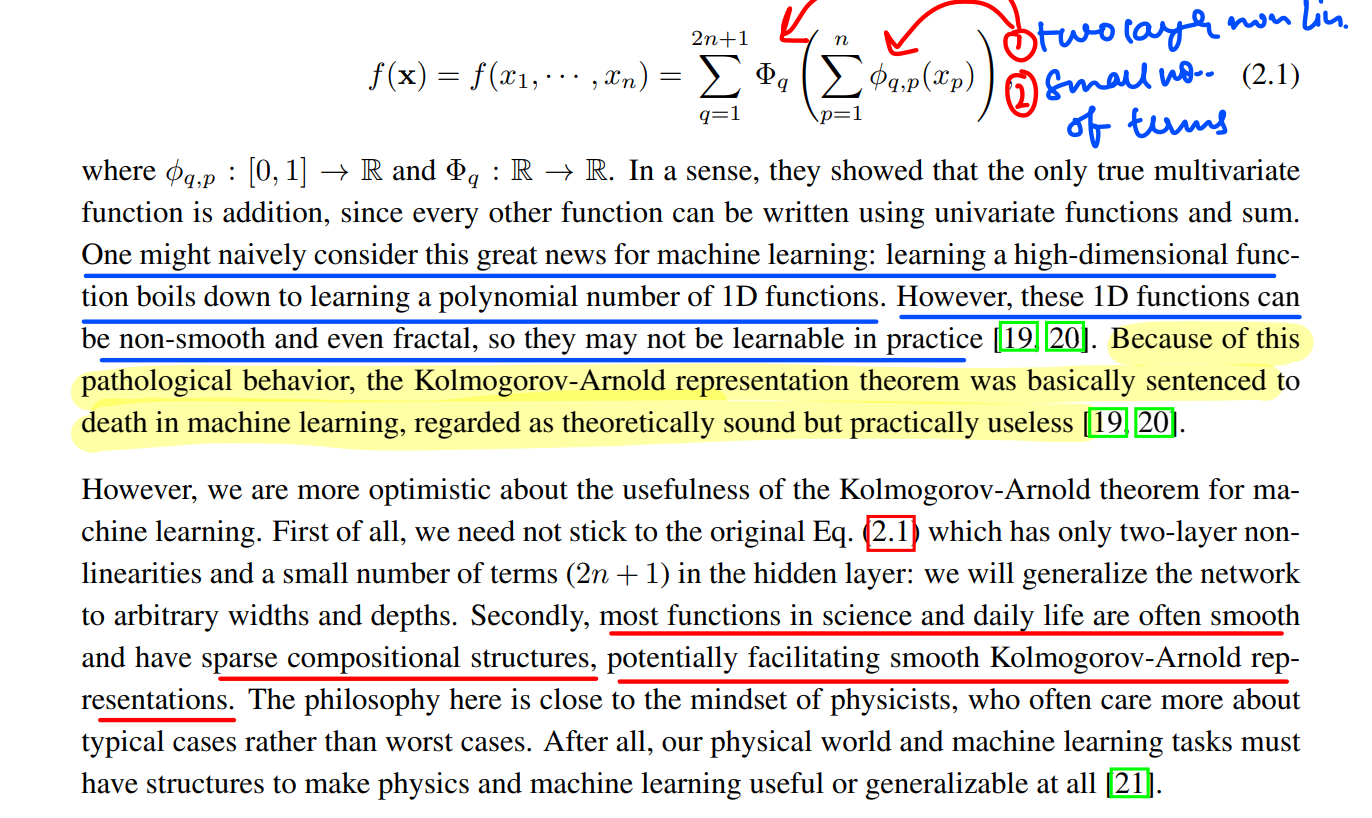
\includegraphics[height=7cm]{image copy 10.png}
    \end{figure}
\end{frame}
\begin{frame}{Architecture}
    \begin{figure}
        \centering
        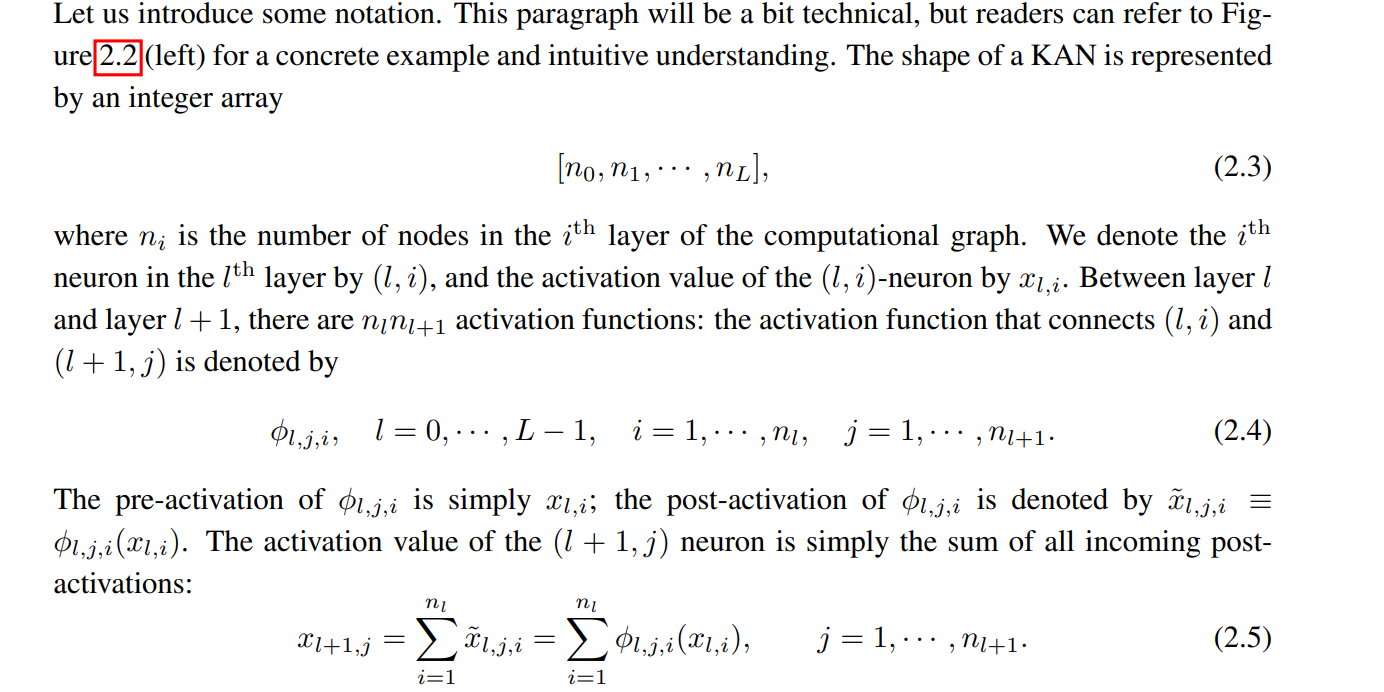
\includegraphics[height=6cm]{image copy 11.png}
    \end{figure}
\end{frame}
\begin{frame}{Architecture}
    \begin{figure}
        \centering
        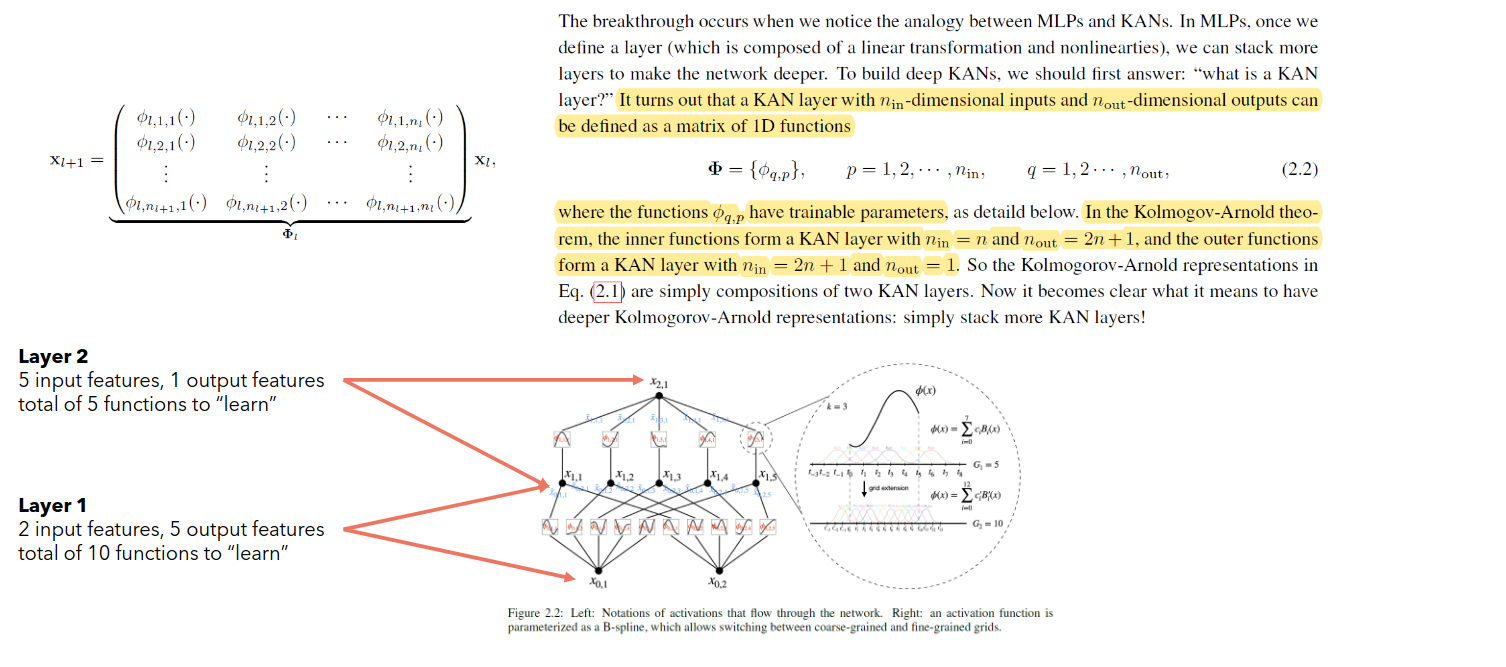
\includegraphics[height=7cm]{image copy 9.png}
    \end{figure}
\end{frame}
\begin{frame}{Example KAN}
    \begin{figure}
        \centering
        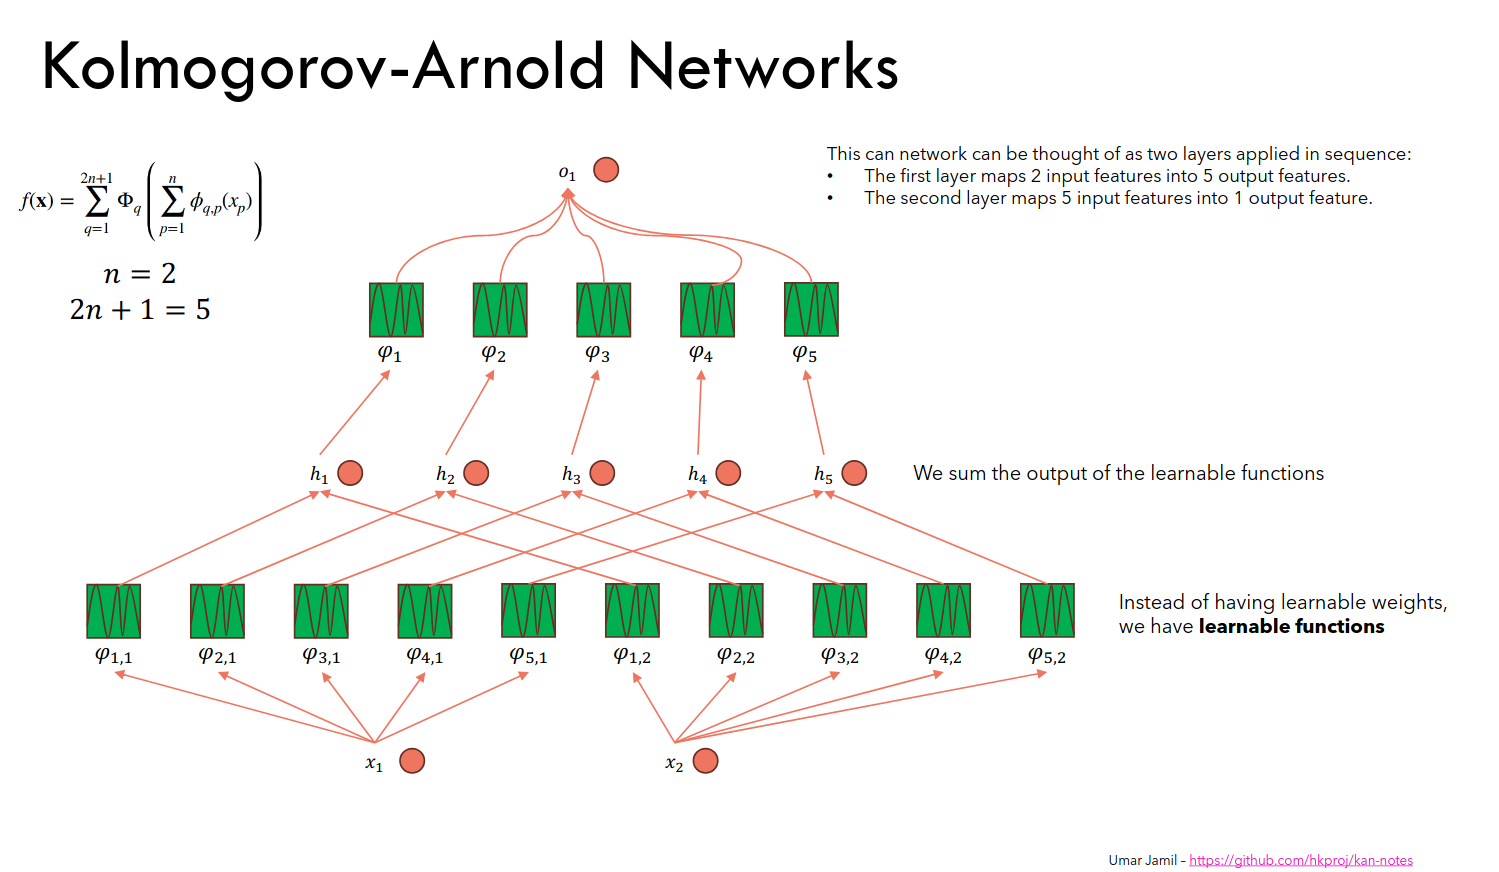
\includegraphics[height=7cm]{image copy 8.png}
    \end{figure}
\end{frame}
\begin{frame}{Example KAN}
    \begin{figure}
        \centering
        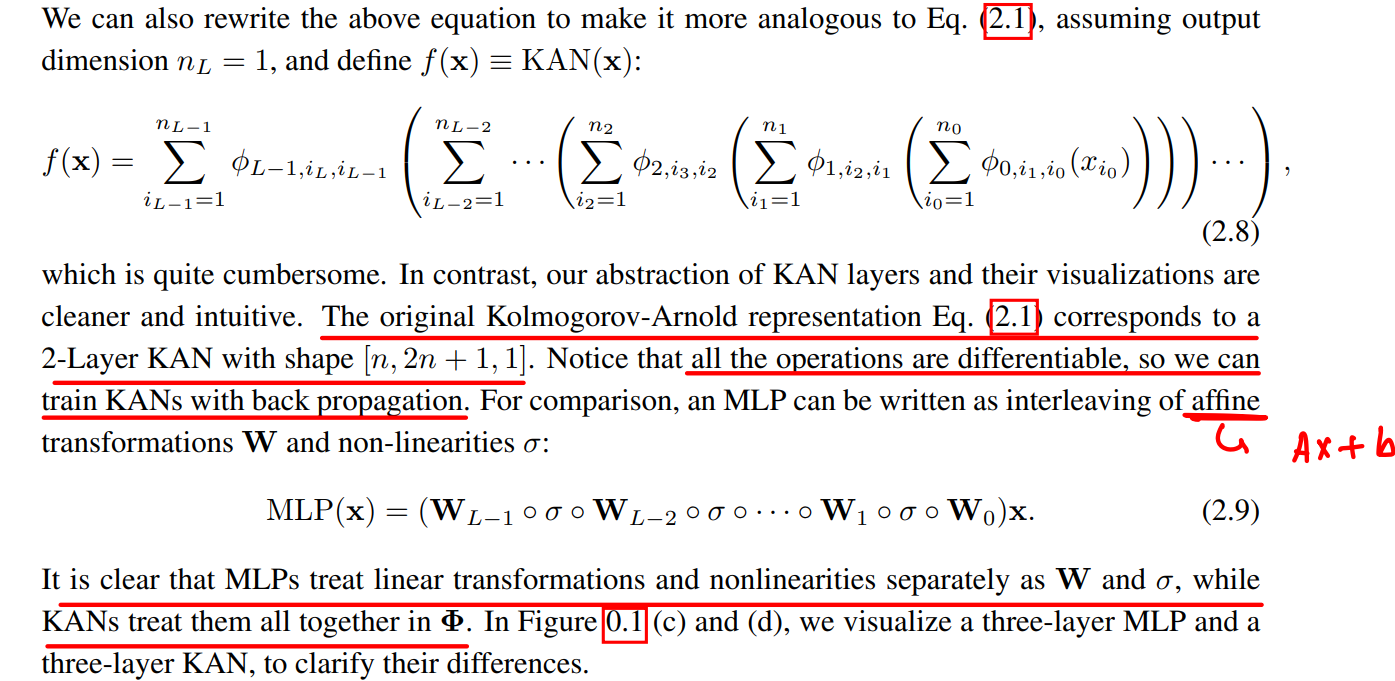
\includegraphics[height=6cm]{image copy 12.png}
    \end{figure}
\end{frame}
\begin{frame}
    \frametitle<presentation>{Implementation}
    \begin{figure}
        \centering
        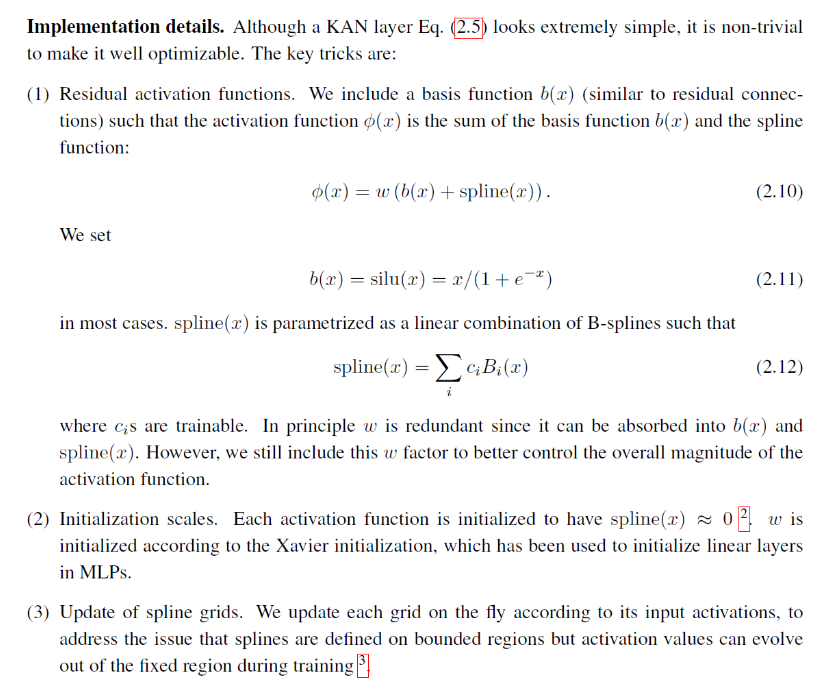
\includegraphics[height=7cm]{image copy 13.png}
    \end{figure}
\end{frame}
\begin{frame}
    \frametitle<presentation>{Implementation}
    (2) This is done by drawing B-spline coefficients $c_i ~ N(0, \sigma^2 )$ with a small $\sigma$, typically we set $\sigma = 0.1$.

    (3) Other possibilities are: (a) the grid is learnable with gradient descent, e.g., Hongyi Xu; (b) use normalization such
    that the input range is fixed. We tried (b) at first but its performance is inferior to our current approach.
\end{frame}\begin{frame}
    \frametitle<presentation>{Parameter Count}
    For a network of:
    \begin{itemize}
        \item depth $L$
        \item all layers of equal width $N$
        \item each spline of order $k$ on a grid of size $G+1$ i.e. $G$ intervals
    \end{itemize}
    The total number of parameters is: $O(N^2L(G+k)) ~ O(N^2L(G))$.

    In contrast, MLP has $O(N^2L)$ parameters.

    Well good news is $N$ is pretty low for KANs compared to MLPs.

    For 1D problems, $N=L=1$ i.e. nothing but a spline approximation.

    For higher dimensions, generalization behaviour of KANs is stated in the theorem below.
\end{frame}
\begin{frame}
    \frametitle<presentation>{Approximation Theory, KAT}
    \begin{figure}
        \centering
        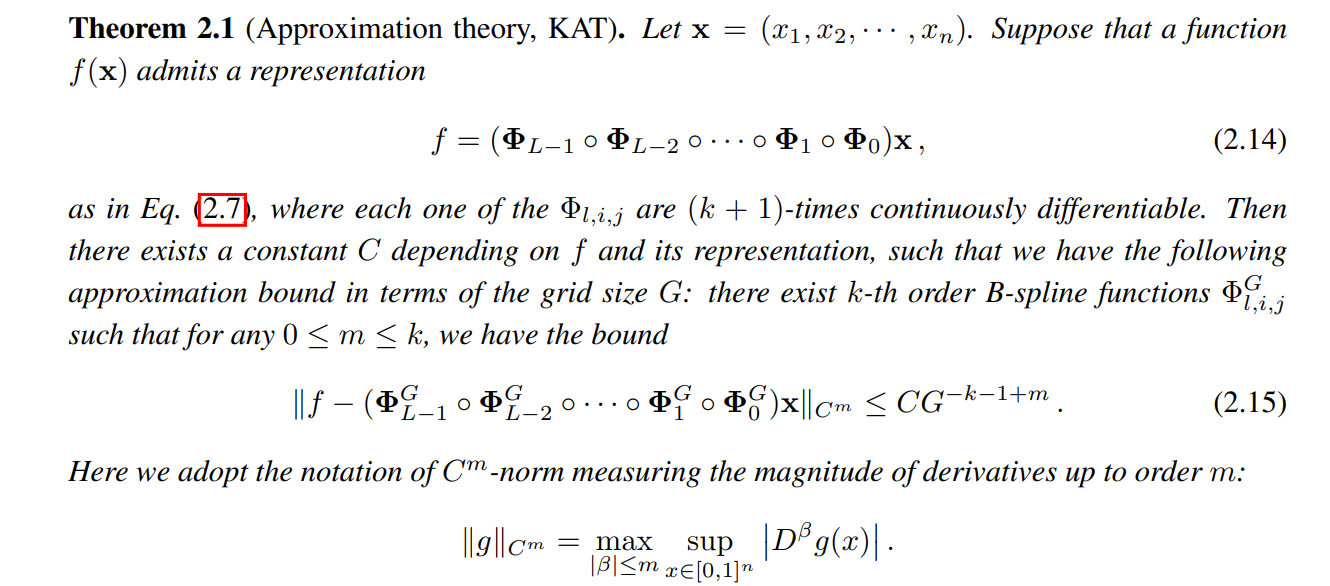
\includegraphics[height=5cm]{image copy 15.png}
    \end{figure}
\end{frame}
\begin{frame}
    \frametitle<presentation>{Inferences from Approximation Theory}
    \begin{figure}
        \centering
        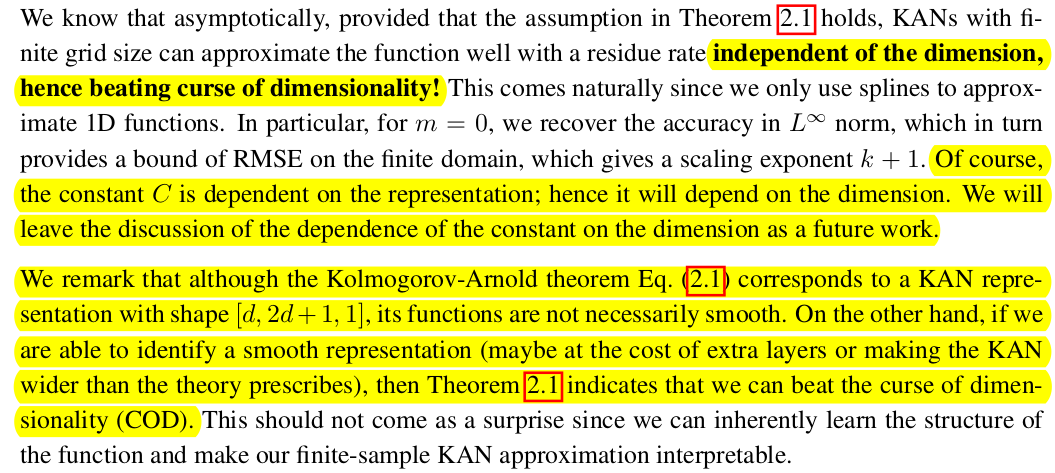
\includegraphics[height=5cm]{image copy 17.png}
    \end{figure}
\end{frame}
\begin{frame}
    \frametitle<presentation>{Neural Scaling Laws}
    \textbf{Neural Scaling Laws:} The test loss \( \ell \) decreases with more model parameters \( N \) following the law \( \ell \propto N^{-\alpha} \), where \( \alpha \) is the scaling exponent. A larger \( \alpha \) indicates better improvement by scaling the model.

    \textbf{Theories for Predicting \( \alpha \):} Sharma \& Kaplan:Suggest that \( \alpha \) is related to the intrinsic dimensionality \( d \) of the input manifold.
    \begin{itemize}
        \item \textbf{Standard Approximation Theory:} For a piecewise polynomial of order \( k \), \( \alpha = \frac{k+1}{d} \). This suffers from the curse of dimensionality.
    \end{itemize}

    \textbf{Alternative Approaches:}
    \begin{itemize}
        \item \textbf{Michaud et al.:} Found \( \alpha = \frac{k+1}{d^*} \), with \( d^* = 2 \) being the maximum arity. They considered only unary and binary functions.
        \item \textbf{Poggio et al.:} Showed that for function classes \( W_m \) with continuous derivatives up to order \( m \), \( \alpha = \frac{m}{2} \).
    \end{itemize}
\end{frame}
\begin{frame}
    \frametitle<presentation>{Neural Scaling Laws}
    \textbf{Approaches for (KANs):}
    \begin{itemize}
        \item \textbf{Proposed Approach:} Decomposes high-dimensional functions into several 1D functions, resulting in \( \alpha = k + 1 \), with \( k = 3 \) for cubic splines, yielding \( \alpha = 4 \).
        \item \textbf{Empirical Validation:} Section 3.1 confirms \( \alpha = 4 \) for KANs, while traditional MLPs have shown slower bounds, like \( \alpha = 1 \).
    \end{itemize}
    \begin{figure}
        \centering
        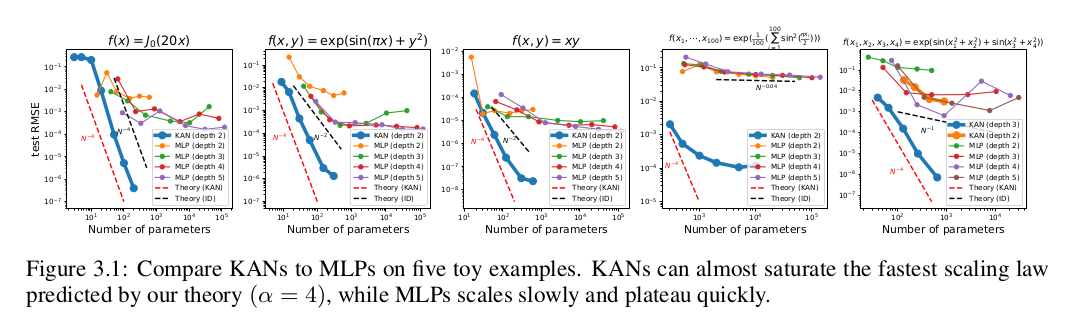
\includegraphics[height=4cm]{image copy 18.png}
    \end{figure}
\end{frame}
\begin{frame}
    \frametitle<presentation>{KAT vs UAT}
    \textbf{Universal Approximation Theorem (UAT):}
    \begin{itemize}
        \item Justifies the power of fully-connected neural networks, stating that a two-layer network with \( k > N(\epsilon) \) neurons can approximate any function within an error \( \epsilon \).
        \item However, UAT does not provide a bound on how \( N(\epsilon) \) scales with \( \epsilon \), leading to COD.
        \item In some cases, \( N \) grows exponentially with the dimensionality \( d \).
    \end{itemize}

    \textbf{Kolmogorov-Arnold Theorem (KAT) vs UAT:}
    \begin{itemize}
        \item KAT leverages the intrinsic low-dimensional representation of functions, unlike MLPs under UAT.
        \item KAT allows for quantifying approximation errors in compositional spaces, offering advantages over UAT.
    \end{itemize}
\end{frame}
\begin{frame}
    \begin{itemize}
        \item Generalization error bounds for finite samples in a similar space have been studied, showing that MLPs with ReLU activations face difficulties in overcoming the COD.
        \item Nonlinear \( n \)-widths theory suggests that MLPs with ReLU activations can achieve a tight rate, but cannot beat the COD in general function spaces like Sobolev or Besov spaces.
    \end{itemize}
    \textbf{Implications of KAT:}
    \begin{itemize}
        \item KAT motivates the use of compositional structures for functions commonly encountered in practice and science, helping to overcome the COD.
        \item This allows the use of smaller architectures in practice, as general nonlinear activation functions are learned.
        \item In contrast, ReLU MLPs may require a depth of at least \( \log n \) to achieve the desired rate, where \( n \) is the number of samples.
        \item KANs are shown to be better aligned with symbolic functions compared to MLPs.
    \end{itemize}
\end{frame}
\begin{frame}
    \frametitle<presentation>{Grid Extension}
    \textbf{Fine-Graining in KANs:} KANs can achieve arbitrarily accurate approximations by refining the grid, a process called "fine-graining." This is a key advantage over MLPs, which lack the concept of grid refinement.

    \textbf{Efficiency:} Unlike MLPs, where increasing width and depth can improve performance but is computationally expensive, KANs can be efficiently enhanced by simply refining the spline grids without retraining from scratch.
\end{frame}
\begin{frame}
    \frametitle<presentation>{How to do Grid Extension}
    We begin with a coarse grid approximation of a 1D function \( f(x) \) defined on the interval \([a, b]\). The grid has \( G_1 \) intervals, with grid points \( \{t_0 = a, t_1, t_2, \dots, t_{G_1} = b\} \), and B-spline basis functions of order \( k \), denoted by \( B_i(x) \).

    The function \( f(x) \) on the coarse grid is approximated as:
    \[
        f_{\text{coarse}}(x) = \sum_{i=0}^{G_1+k-1} c_i B_i(x)
    \]
    We then extend this to a finer grid with \( G_2 \) intervals, introducing additional grid points \( \{t_{G_1+1}, t_{G_1+2}, \dots, t_{G_2+k}\} \). The new approximation on the fine grid is:
    \[
        f_{\text{fine}}(x) = \sum_{j=0}^{G_2+k-1} c'_j B'_j(x)
    \]
    Note that the $i^{th}$ B-spline i.e. $B_i(x)$ is non zero only in the interval $[t_{-k+i}, t_{i+1}]$.
\end{frame}
\begin{frame}
    \frametitle<presentation>{How to do Grid Extension}
    The new coefficients \( \{c'_j\} \) are determined by minimizing the distance:
    \[
        \{c'_j\} = \argmin_{\{c'_j\}} \mathbb{E}_{x \sim p(x)} \left( \sum_{j=0}^{G_2+k-1} c'_j B'_j(x) - \sum_{i=0}^{G_1+k-1} c_i B_i(x) \right)^2
    \]
    This can be implemented using the least squares algorithm.
\end{frame}
\begin{frame}
    \frametitle<presentation>{Staircase like loss curves}
    We use a toy example \( f(x, y) = \exp(\sin(\pi x) + y^2) \) to demonstrate the effect of grid extension. In Figure 2.3 (top left), we show the train and test RMSE for a \([2, 5, 1]\) KAN. The number of grid points starts at 3, increases to a higher value every 200 L-BFGS steps, ending up with 1000 grid points.

    It is clear that every time fine graining happens, the training loss drops faster than before (except for the finest grid with 1000 points, where optimization ceases to work probably due to bad loss landscapes). However, the test losses first go down, then go up, displaying a U-shape due to the bias-variance tradeoff (underfitting vs. overfitting).

    We conjecture that the optimal test loss is achieved at the interpolation threshold when the number of parameters matches the number of data points. Since our training samples are 1000 and the total parameters of a \([2, 5, 1]\) KAN is \(15G\) (where \(G\) is the number of grid intervals), we expect the interpolation threshold to be \( G = \frac{1000}{15} \approx 67 \), which roughly agrees with our experimentally observed value \( G \sim 50 \).
\end{frame}
\begin{frame}
    \frametitle<presentation>{Staircase like loss curves}
    \begin{figure}
        \centering
        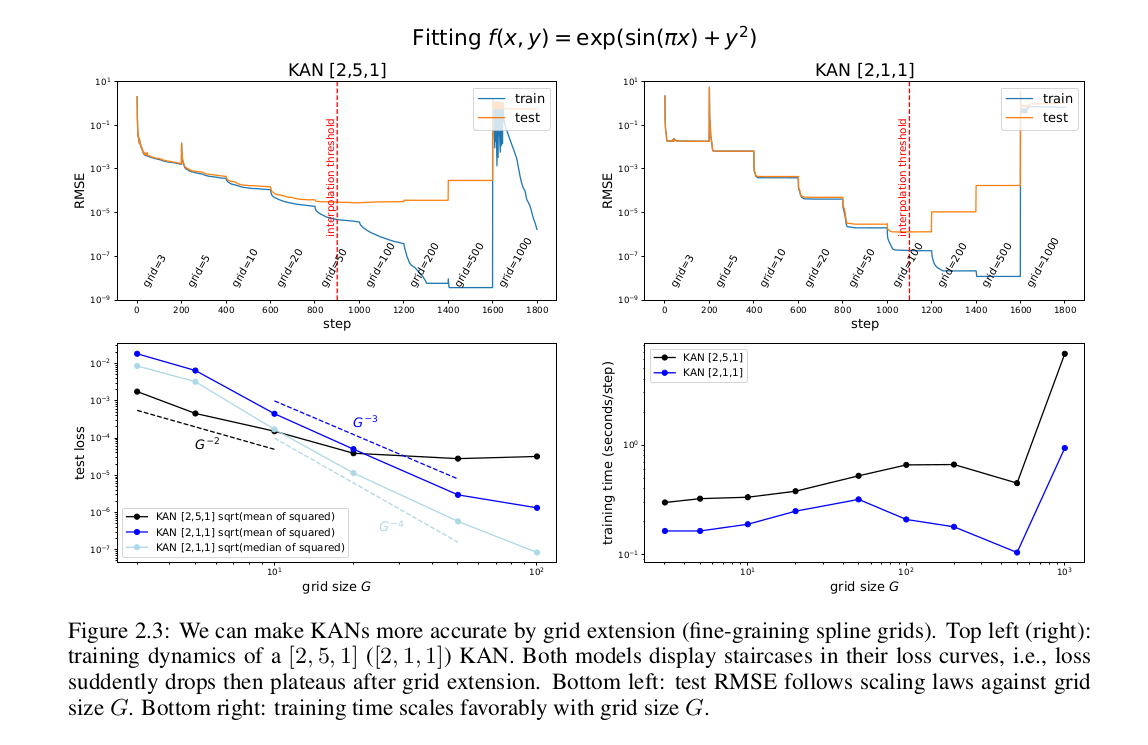
\includegraphics[height=7cm]{image copy 20.png}
    \end{figure}
\end{frame}
\begin{frame}
    \frametitle<presentation>{Small KANs generalize better}
    As we can see above, small KANs generalize better: A [2,1,1][2,1,1] KAN achieves lower test losses and better generalization than a larger [2,5,1][2,5,1] KAN. This highlights the \textbf{importance of choosing minimal architectures}, which can be discovered via regularization and pruning (discussed in Section 2.5).
\end{frame}
\begin{frame}
    \frametitle<presentation>{Scaling laws emperically}

\end{frame}
% Results --- --- --- --- --- --- --- --- --- --- ---
\section{Results}
\begin{frame}
    \begin{itemize}
        \item different themes
        \item different themes
        \item different themes
        \item different themes
    \end{itemize}
\end{frame}


% --- Thank you slide ---
\begin{frame}
    \begin{center}
        {End}
        \vspace{1cm}

        MAS\\[1em]
    \end{center}
\end{frame}

\end{document}